\documentclass{article}
\usepackage[utf8]{inputenc}
\usepackage[icelandic]{babel}
\usepackage[T1]{fontenc}
\usepackage{graphicx}
\usepackage{mathtools}
\usepackage{amsmath}
\usepackage{amssymb}
\usepackage{minted}


\graphicspath{ {./} }
\title{Titill - Áfangi}
\author{ttb3@hi.is}
\date{\today}


\begin{document}
\maketitle


\section{}
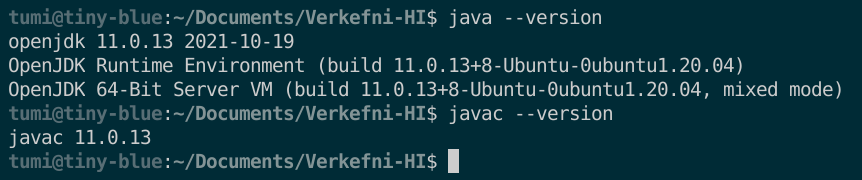
\includegraphics[scale=0.4]{javas.png}

\section{}
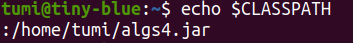
\includegraphics[scale=1]{CLASSPATH.png}

\section{}
Ég hef lesið og skilið reglurnar um afritun lausna

\newpage
\section{}
\begin{minted}{java}
    import edu.princeton.cs.algs4.StdDraw;
    import java.awt.Font;

    public class Ugla {
        public static void main(String args[]) {
            Font font = new Font("Arial", Font.BOLD, 25);
            StdDraw.setFont(font);
            StdDraw.text(0.5, 0.6, "Ég heiti Þorvaldur Tumi Baldursson");
            StdDraw.setPenColor(StdDraw.RED);
            StdDraw.text(0.5, 0.4, "og netfangið mitt er ttb3@hi.is");
        }
    }
\end{minted}
\begin{center}
    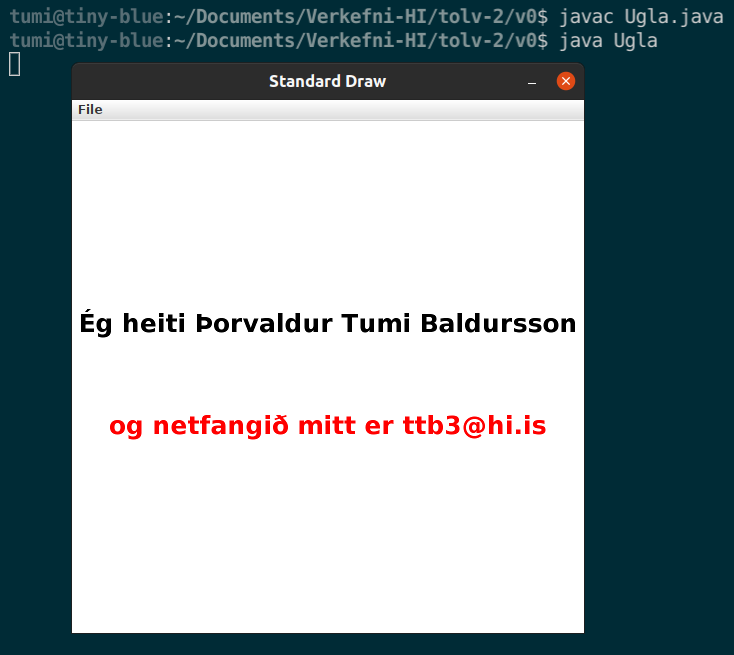
\includegraphics[scale=0.5]{comprun.png}\\
\end{center}

\end{document}